\chapter{System Design Specification}
\section{System Architecture}
\paragraph{}SMPTMS follows a three-tier client-server architecture. The presentation layer is built on Next.js 14 with the App Router, running in the user's browser as a React-based single-page application. The application layer handles all business logic --- including tax calculation, authentication middleware, payment processing, and webhook verification --- through Next.js API routes and server components executing in a Node.js runtime environment. The data layer resides on Supabase, which manages a PostgreSQL relational database, file storage for receipt PDFs, and real-time data subscriptions.

\paragraph{}All three tiers communicate exclusively over HTTPS. Citizens and administrators access the same Vercel deployment at smptms.vercel.app but are presented with entirely different interfaces based on their assigned role, which is verified on every request through Supabase Auth middleware running at the edge.

\paragraph{}The payment flow operates through a dedicated sub-process: when a citizen initiates payment, the Next.js API creates a Razorpay order object, the citizen completes payment on Razorpay's hosted checkout page, and Razorpay sends a signed webhook callback to the server. The server verifies the cryptographic signature before updating the property payment status in Supabase and generating the receipt document.

\section{Module Decomposition Description}
\paragraph{}SMPTMS is organized into four primary modules, each owned and developed by a dedicated team member:

\textbf{Module 1 --- User Management (Khushal Jangid):} Handles user authentication, role-based access control (Citizen/Admin), session management via Supabase Auth, and the citizen-facing dashboard displaying property portfolio and dues.

\textbf{Module 2 --- Tax Calculation (Gaurav Pratap Singh):} Covers the Supabase schema design for property records and tax assessments, DLC rate configuration per zone, automated tax formula implementation (Tax = Plot Area x DLC Rate / 2000), and the assessment approval workflow for administrators.

\textbf{Module 3 --- Testing Module (Kapil Jarwal):} Encompasses the complete quality assurance pipeline including Postman API testing, integration testing across all modules, automated test case development, Vercel deployment management, and bug tracking documentation.

\textbf{Module 4 --- Surveying / GIS (Himanshu Meena):} Manages the Leaflet.js GIS map integration with real Jaipur coordinates, colour-coded property marker rendering, ward-wise and zone-wise filtering, Google Maps satellite tile toggle, and survey data upload with version history tracking.

\section{High Level Design Diagrams}
\subsection{Use Case Diagram}
\begin{figure}[H]
  \centering
    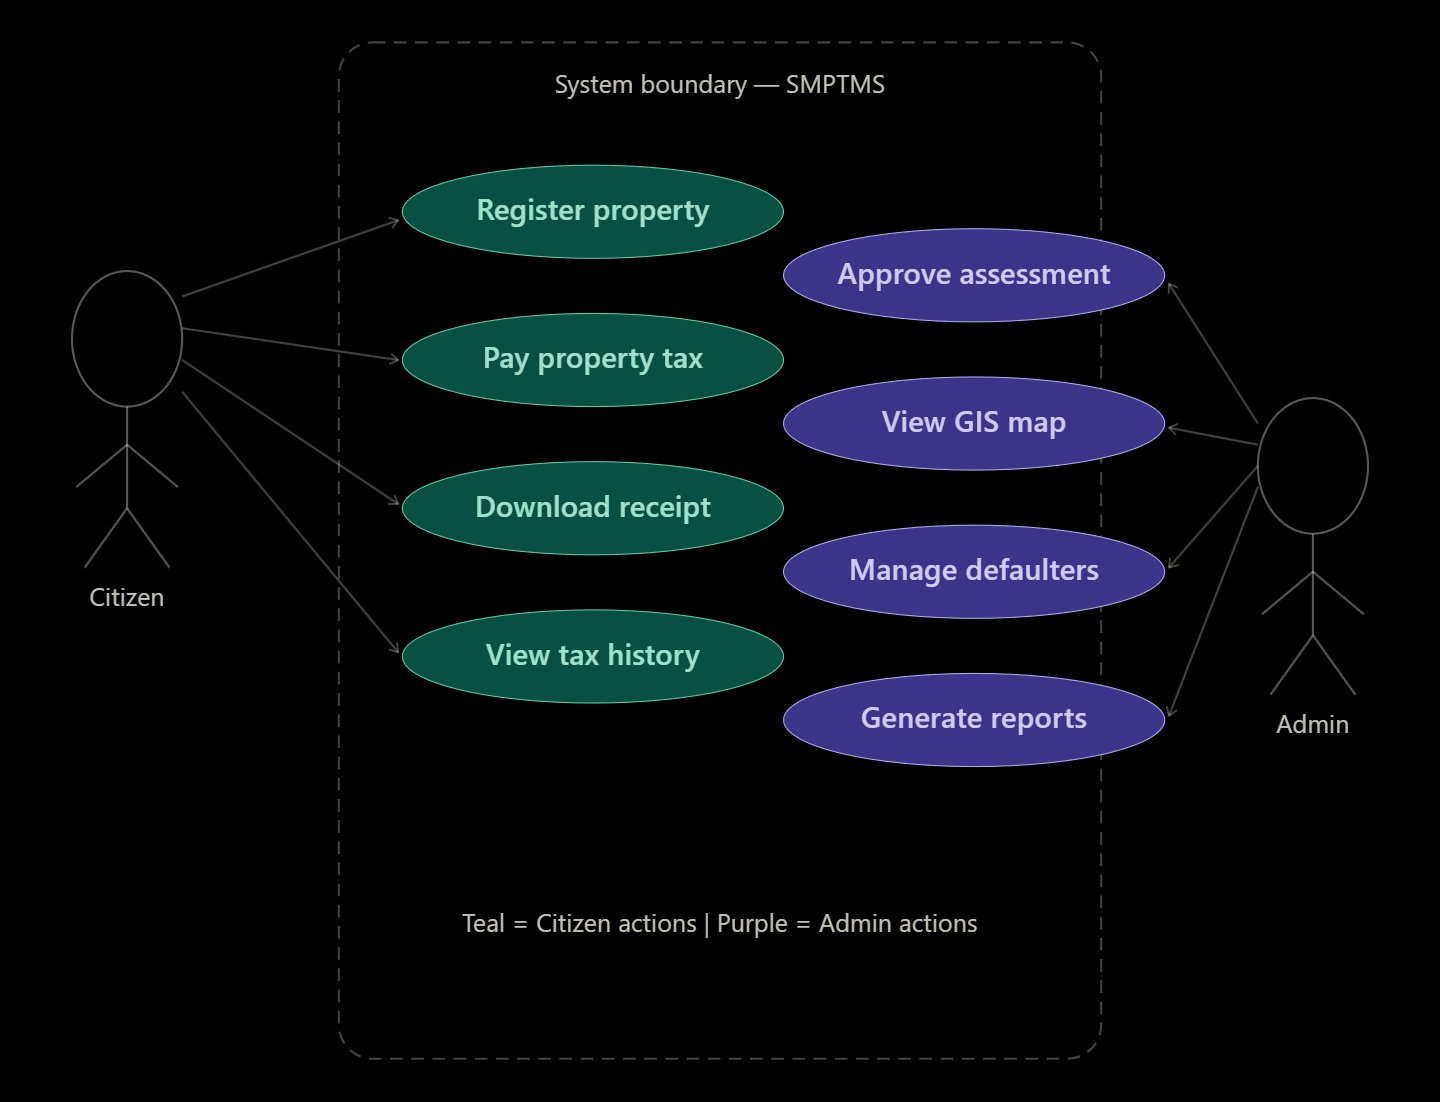
\includegraphics[width=0.85\textwidth]{project/images/usecase.png}\\
  \caption{Use Case Diagram of SMPTMS}
\end{figure}

\subsection{Activity Diagram}
\begin{figure}[H]
  \centering
    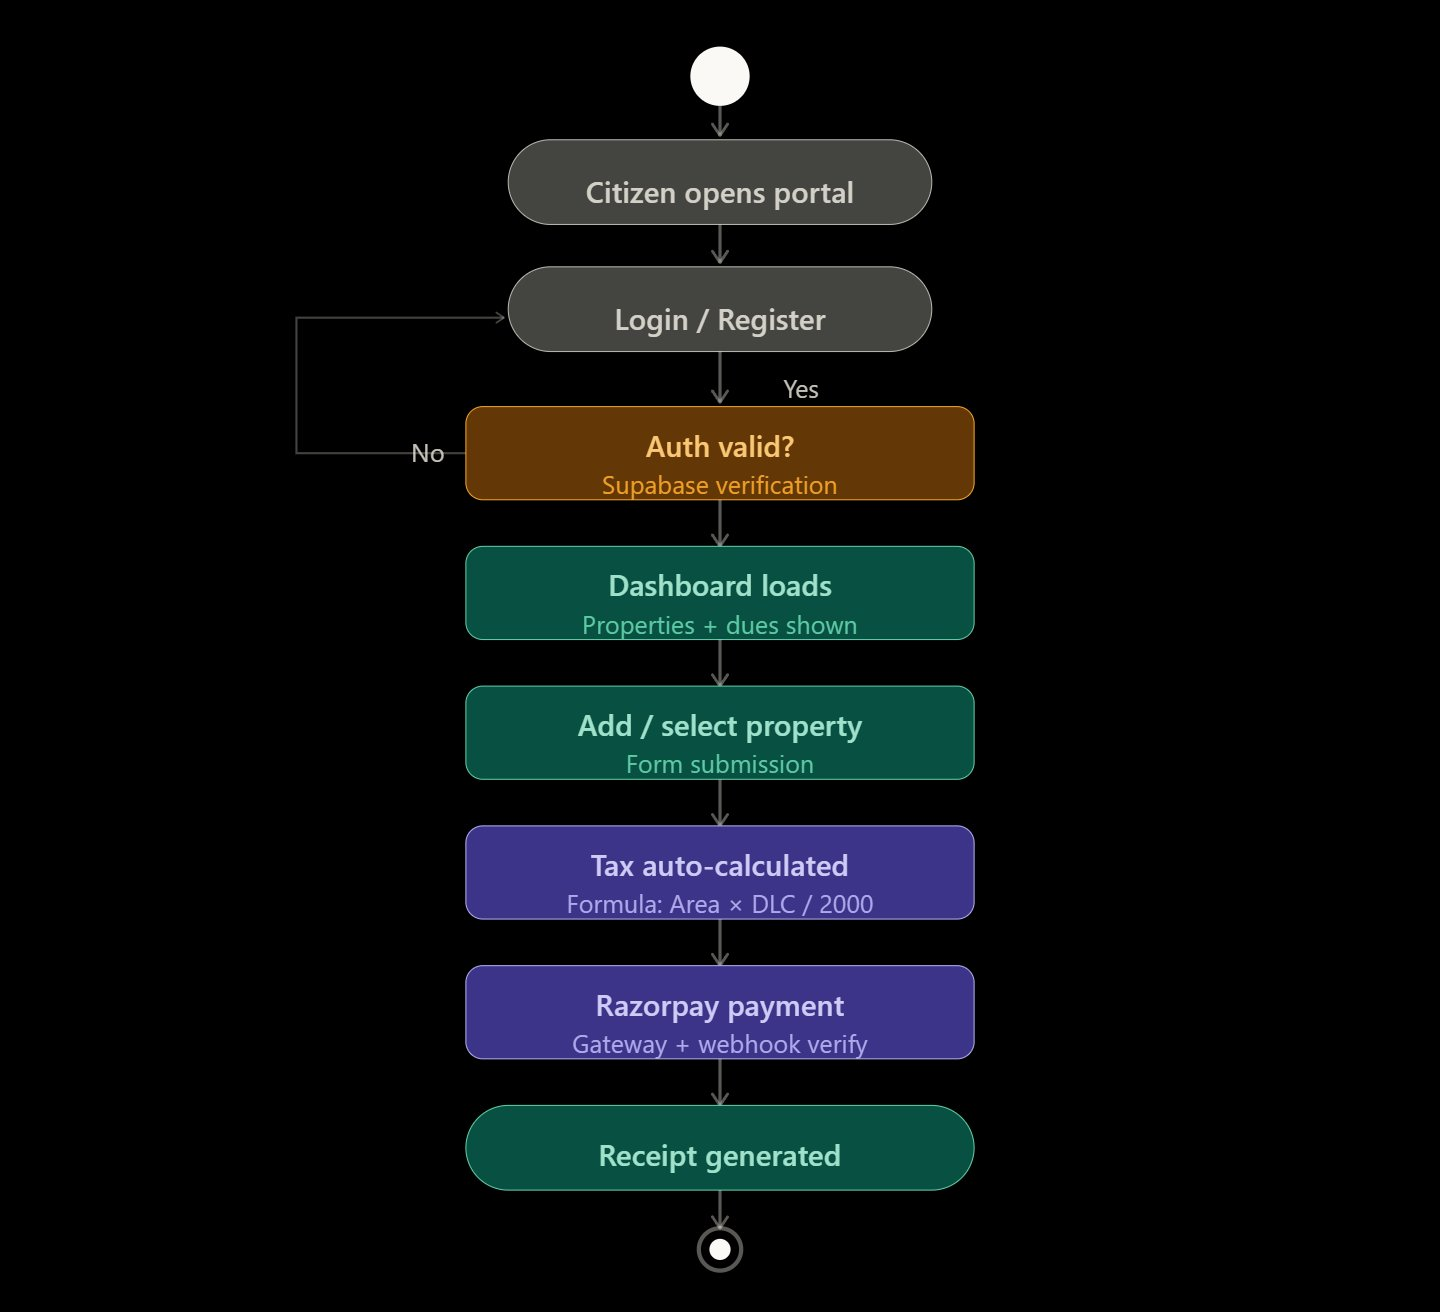
\includegraphics[width=0.75\textwidth]{project/images/activity.png}\\
  \caption{Activity Diagram -- Citizen Tax Payment Flow}
\end{figure}

\subsection{Data-Flow Diagram}
\begin{figure}[H]
  \centering
    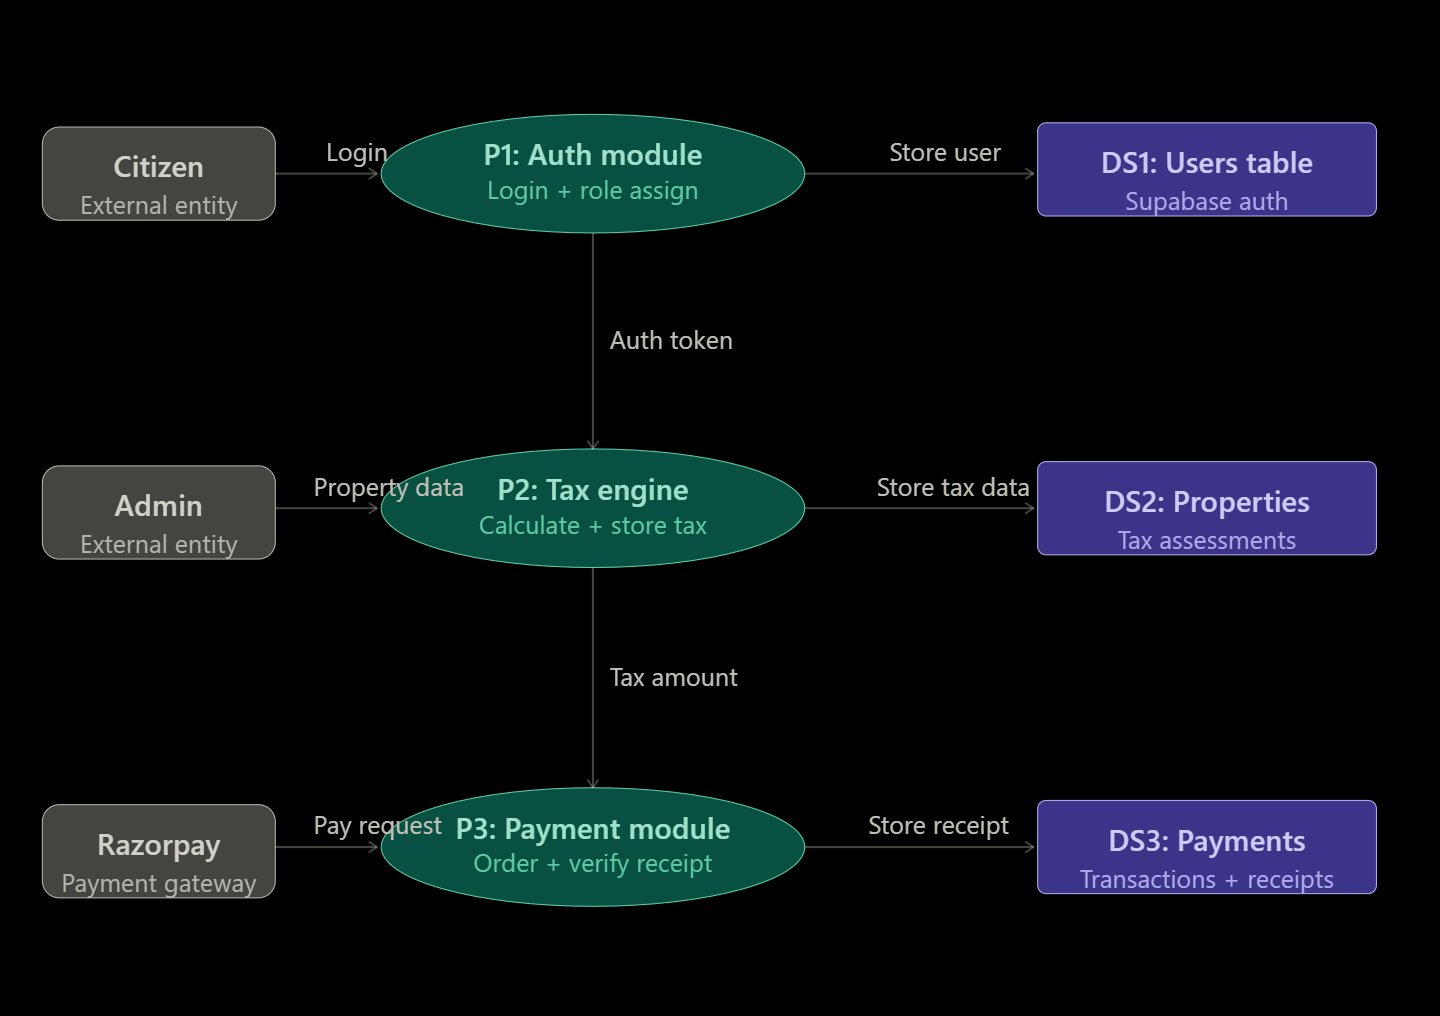
\includegraphics[width=0.85\textwidth]{project/images/data-sync.png}\\
  \caption{Data-Flow Diagram of SMPTMS}
\end{figure}

\subsection{Class Diagram}
\begin{figure}[H]
  \centering
    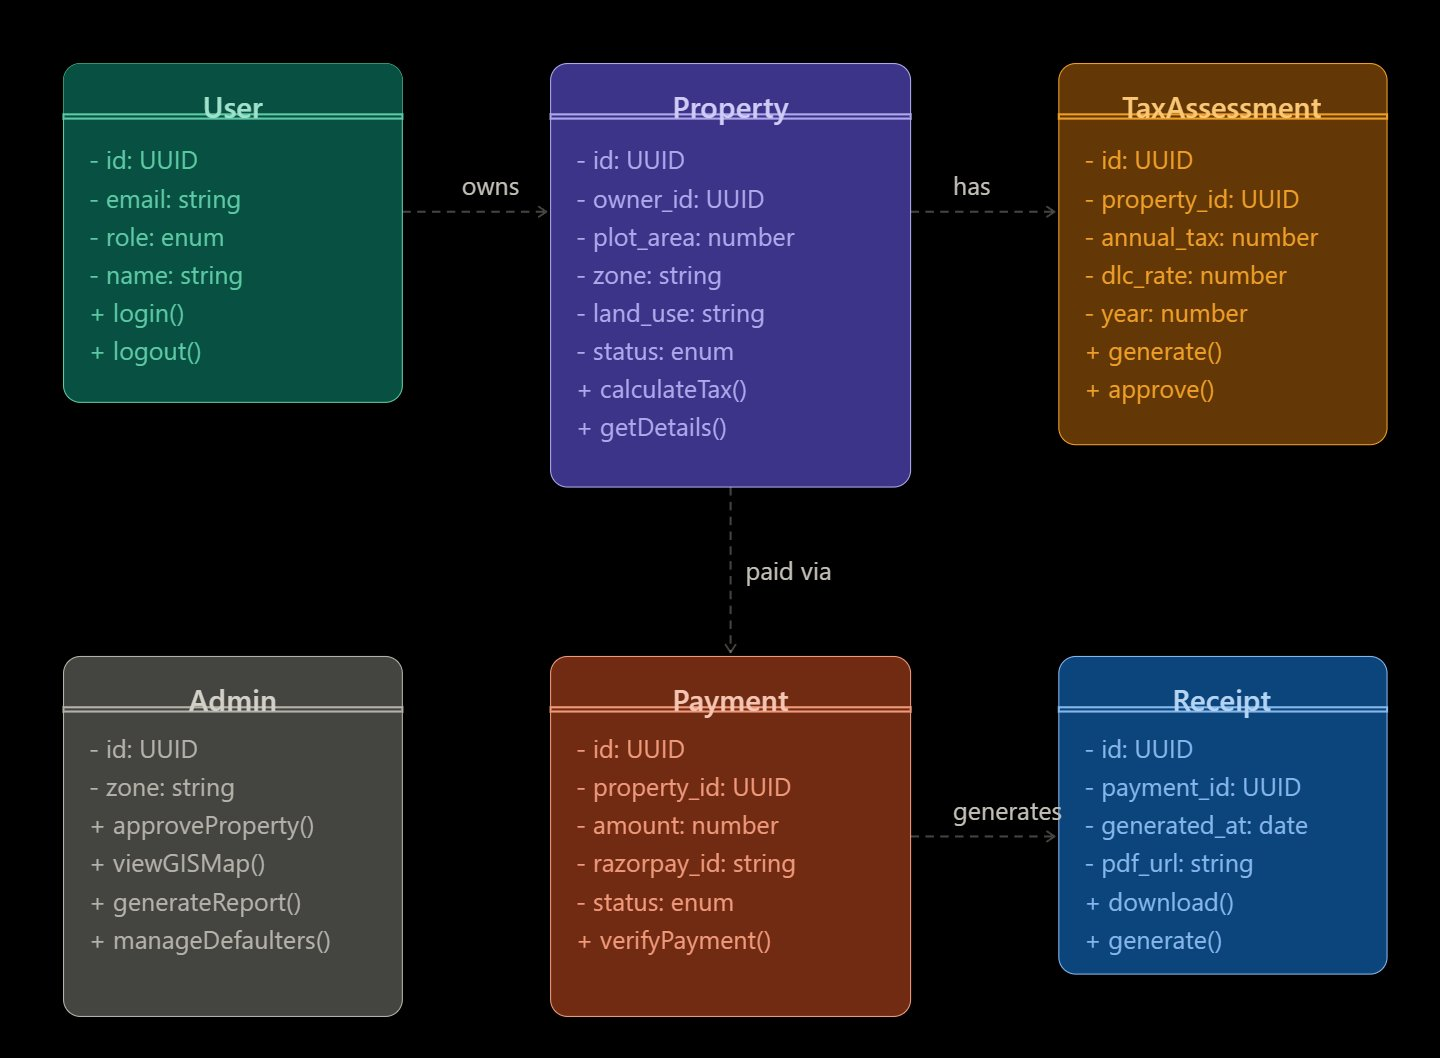
\includegraphics[width=0.85\textwidth]{project/images/classDiagram.png}\\
  \caption{Class Diagram of SMPTMS}
\end{figure}

\subsection{Sequence Diagram}
\begin{figure}[H]
  \centering
    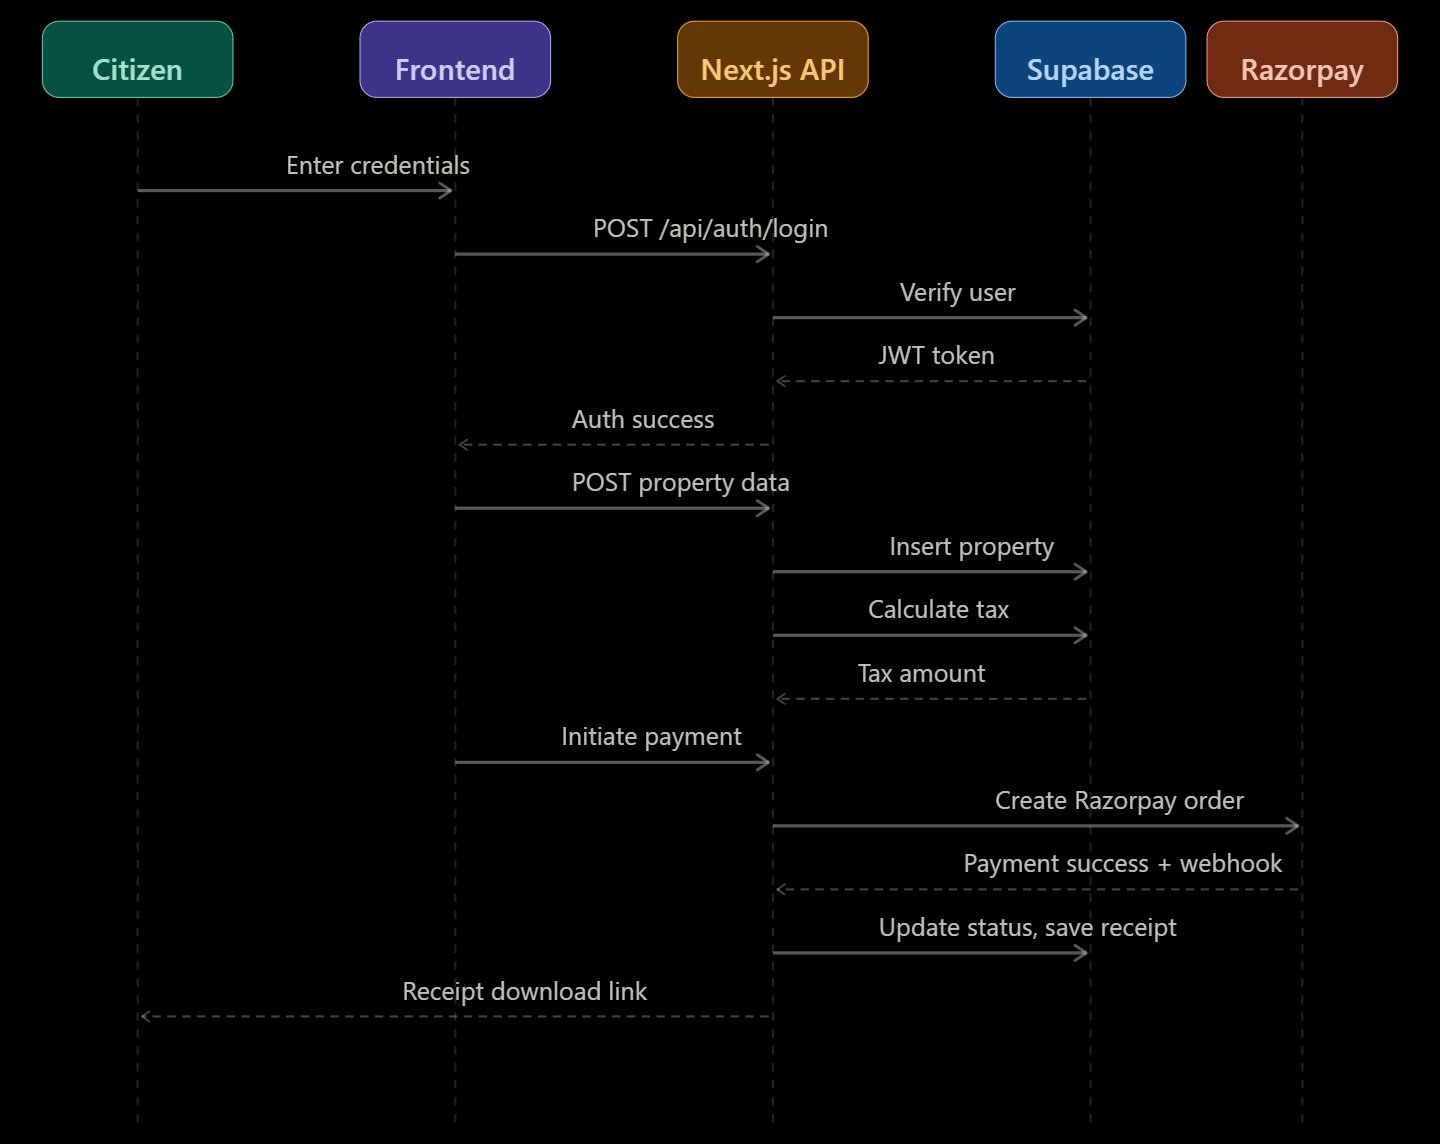
\includegraphics[width=0.85\textwidth]{project/images/seq.png}\\
  \caption{Sequence Diagram -- Payment Processing Flow}
\end{figure}
